% BREDEX LaTeX Template
%  \documentclass is either ``bxreport'' or ``bxarticle''
%                 option is bxpaper
%% \documentclass{bxarticle}
%% % ----------------------------------------------------------------------
%% \begin{document}
%% \title{}
%% \author{}
%% % \author*{Hauptautor}{Liste der Nebenautoren}
%% \maketitle
%% % ----------------------------------------------------------------------
%% \bxversion{0.1}
%% %\bxdocinfo{STATUS}{freigegeben durch}{freigegeben am}{Verteilerliste}
%% \bxdocinfo{DRAFT}{}{}{}
%% % ----------------------------------------------------------------------

%% \end{document}

\index{Project!Properties}
\index{Edit!Project Properties}
You can open the \gdproject{} properties dialog (\bxfigref{projectsettingsdialog}) via:\\
\bxmenu{Test}{Properties}{}

\begin{figure}[h]
\begin{center}
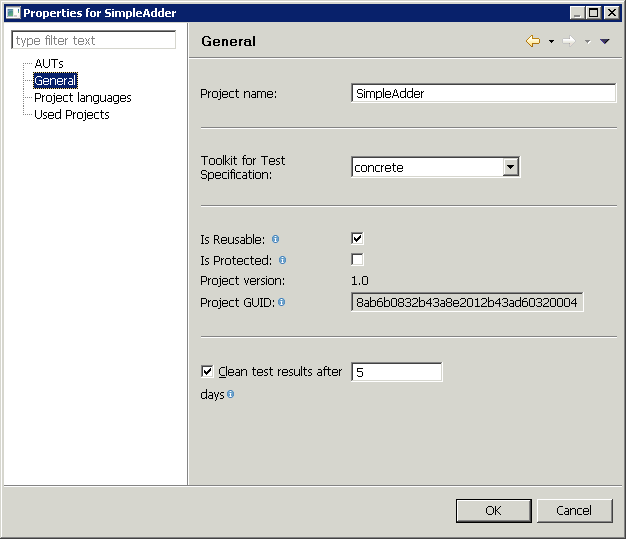
\includegraphics[width=12.5cm]{Tasks/Projects/PS/general_projproperties}
\caption{Project Properties Dialog}
\label{projectsettingsdialog}
\end{center}
\end{figure}

The \gdproject{} properties dialog  lets you see and, in some cases, edit information about:
\begin{enumerate}
\item the \gdproject{} in general \bxpref{ProjPropertiesGeneral}.
\item the \gdproject{} languages \bxpref{ProjPropertiesLanguage}.
\item the \gdauts{} \bxpref{ProjPropertiesEditAUT}.
\item the \gdprojects{} that you have reused in this \gdproject{} \bxpref{reuseproject}. 
\item any extensions you have added for the \gdproject{} \bxpref{TasksBasicExtension}.
\end{enumerate}

\subsubsection{Editing general \gdproject{} properties}
\gdhelpid{projectSettingsPageContextId}{Project Properties}
\label{ProjPropertiesGeneral}
Select \bxcaption{General} from the tree on the left-hand side of the \gdproject{} properties dialog. In the screen that appears, you can:
\begin{enumerate}
\item Edit the \gdproject{} name. 
\item Edit the toolkit used by the \gdproject{} (see the following section \bxpref{ProjPropertiesChangingToolkit} for details on this). 
\item Edit whether the \gdproject{} can be referenced (reused) in other \gdprojects{}.
\item Edit the protected status of the \gdproject{}. A protected \gdproject{} does not allow deletion of \gdcases{} or editing of parameters. 
\item See the \gdproject{} version. This is useful if you have more than one version of a \gdproject{}. 
\item See the GUID (global unit identification). This is a unique ID for the \gdproject{}. 
\item Specify how often the full test result details \bxpref{TasksReopenTestResult} should be automatically deleted from the \gddb{}.
\end{enumerate}

\subsubsection{Changing the toolkit settings for a \gdproject{}}
\label{ProjPropertiesChangingToolkit}
If you want to change the toolkit of a \gdproject{} in the \gdproject{} properties dialog, the following rules apply:
\begin{enumerate}
\item You can change at any time from the \bxname{concrete} toolkits to a more specific toolkit (e.g. RCP, HTML). 
\item If your previous choice of toolkit was RCP, SWT or HTML, you can only change to another toolkit if your \gdproject{} does not use any components specific to the originally chosen toolkit. 
\end{enumerate}

\subsubsection{Editing the languages for a \gdproject}
\gdhelpid{projectSettingsPageContextId}{Project Properties}
\label{ProjPropertiesLanguage}
To see and edit the \gdproject{} languages, select \bxcaption{Project languages} from the tree on the left-hand side of the \gdproject{} properties dialog. 

You can add and remove \gdproject{} languages and change the default language in this screen. 
 
\bxtipp{You can't delete a language which is being used as an \gdaut{} language.}


\subsubsection{Editing the \gdauts{} in a \gdproject{}}
\label{ProjPropertiesEditAUT}
\gdhelpid{autSettingsPageContextId}{Adding/editing AUT's}

To see and edit your \gdauts{} for a \gdproject{},  select \bxcaption{AUTs} from the tree on the left-hand side of the \gdproject{} properties dialog. 

In the screen that appears, you can see any \gdauts{} you have already added to the \gdproject{} (\bxfigref{autsettingsdialog}). You can choose to edit them, delete them or add a new \gdaut{}. 

\begin{figure}[h]
\begin{center}
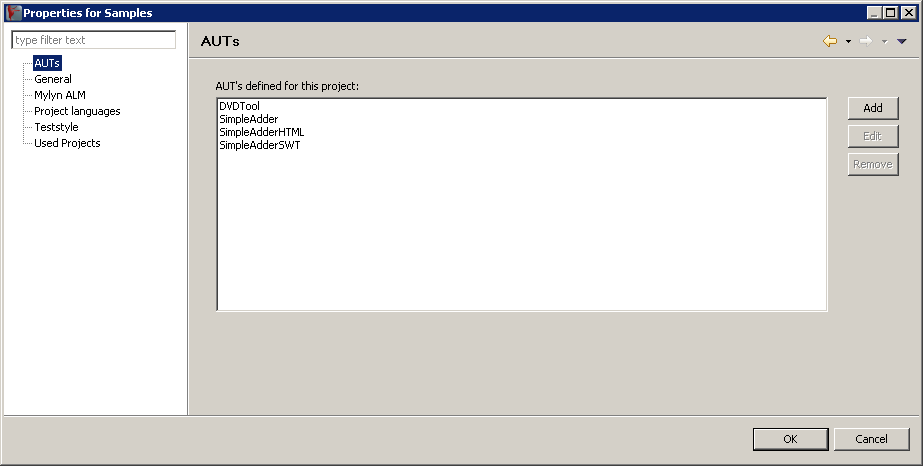
\includegraphics[width=12.5cm]{Tasks/Projects/PS/autsettingsdialog}
\caption{AUT Properties Dialog}
\label{autsettingsdialog}
\end{center}
\end{figure}

Defining and editing \gdauts{} from here involves the same steps as defining  an \gdaut{} in the \gdproject{} wizard \bxpref{Defineaut}. 

\subsubsection{Duplicating \gdaut{} configurations}
\gdhelpid{autConfigSettingWizardPagePageContextId}{Configuring an AUT}
\gdhelpid{autSettingsPageContextId}{Adding/editing AUT's}

You can duplicate an existing \gdaut{} configuration from the \gdproject{} properties dialog:
\begin{enumerate}
\item Select \bxcaption{AUTs} from the tree on the left-hand side of the \gdproject{} properties dialog.
\item Select the \gdaut{} configuration you want to duplicate.
\item Click \bxcaption{Duplicate}.
\item The \gdaut{} configuration dialog will open. The \gdaut{} configuration name and the \gdaut{} ID are automatically changed so that they remain unique. We recommend writing more meaningful names for the configuration and the ID, however. 
\end{enumerate}


\subsubsection{Editing the \gdaut{} configurations in a \gdproject{}}
\label{ProjPropertiesEditAUTConfig}
\gdhelpid{autConfigPropDialogContextId}{Adding/editing AUT configurations}
Select \bxcaption{AUTs} from the tree on the left-hand side of the \gdproject{} properties dialog. 

In the screen that appears, you can see the \gdauts{} you have added to this \gdproject{}. Select the \gdaut{} you want to add a configuration to, and click \bxcaption{Edit}. 

In the next screen there is a box labelled \bxcaption{\gdaut{} configurations}. You can choose to add, edit or delete \gdaut{} configurations. 

Adding and editing \gdaut{} configurations from here involves the same steps as adding an \gdaut{} configuration in the \gdproject{} wizard \bxpref{configuringaut}. 


